\documentclass[11pt]{article}
\usepackage[T1]{fontenc}
\usepackage[utf8]{inputenc}
\usepackage{lmodern,microtype}
\usepackage[margin=1in]{geometry}
\usepackage{amsmath,amssymb,graphicx,booktabs,array,tabularx,longtable}
\usepackage{natbib}
\usepackage[dvipsnames]{xcolor}
\usepackage[colorlinks=true,linkcolor=MidnightBlue,citecolor=MidnightBlue,urlcolor=MidnightBlue]{hyperref}
\usepackage{caption,placeins}
\usepackage{tikz}
\usetikzlibrary{arrows.meta,positioning}
\usepackage{lineno}
\modulolinenumbers[5]
\linenumbers
\newcommand{\model}{PE-RankFormer}
\newcommand{\atone}{\ensuremath{U_1}}
\newcommand{\rhoS}{\ensuremath{\rho_{\mathrm S}}}
\newcommand{\artifact}[1]{\nolinkurl{#1}}
\newcolumntype{Y}{>{\raggedright\arraybackslash}X}
\newcolumntype{P}[1]{>{\raggedright\arraybackslash}p{#1}}
\setlength{\emergencystretch}{2em}
\captionsetup{font=small,labelfont=bf}
\title{From efficiency prediction to pegRNA selection:\\decision-aligned evaluation and source-preserving adaptation of PE-RankFormer}
\author{[Author names and affiliations to be supplied]\\{}[Corresponding author and contact to be supplied]}
\date{Research manuscript --- 12 September 2026}
\begin{document}
\maketitle
\begin{abstract}
Prime-editing efficiency predictors are commonly compared by correlation across measured designs, whereas their practical use requires choosing among alternative pegRNAs for a fixed intended edit. We investigated the relationship between these tasks using \model{}, a sequence model combining paired wild-type/edited representations, context conditioning and ordinal or proportion-based supervision. On the 20,509-row source benchmark, its frozen heterogeneous ensemble achieved Spearman correlation 0.9079 versus 0.8690 for released OptiPrime. Corrected fixed-edit evaluation also favored \model{} on 1,463 informative source decisions: the mean efficiency of the highest-scored candidate was 0.13636 versus 0.12721. However, on an initially reserved external library containing 30,475 eligible decisions, the source-trained ordinal--state-space ensemble retained higher correlation (0.7091 versus 0.6931) but lower top-choice efficiency (0.03627 versus 0.03690; paired difference $-0.00064$, 95\% interval $[-0.00089,-0.00038]$). Audits identified consequential distinctions between decision grouping and batch composition, prediction-head retention and deployed-selector retention, and optimization-seed and label-acquisition replication. Target-supervised ordinal fine-tuning improved top-choice efficiency to 0.04178 versus 0.04020 for unadapted OptiPrime on a separate retrospective library test subset. In 76 subsequent computational fits, stronger optimization controls and repeated label acquisitions removed a simple source-anchoring advantage. A source-balanced teacher-margin constraint improved retention, but constrained adaptation sacrificed target performance and did not outperform OptiPrime at a nominal 1,000-group label budget. These results establish a dataset-specific prediction improvement and a supervised adaptation benefit, while showing why neither implies universally superior design selection. The resulting computational framework evaluates actual deployed decisions, label cost, source retention and evaluation exposure together; independent-study confirmation remains outstanding.
\end{abstract}

\noindent\textbf{Keywords:} prime editing; pegRNA design; state-space models; ordinal regression; domain adaptation; decision evaluation; reproducibility.
\section{Introduction}
Prime editing enables programmable substitutions, insertions and deletions without requiring a donor DNA template or a double-strand break \citep{anzalone2019}. Its practical success depends in part on the choice of prime-editing guide RNA (pegRNA). Alternative spacers, primer-binding sites (PBSs), reverse-transcription templates (RTTs) and guide constructs can produce different outcomes for the same intended edit. A useful computational method must therefore order candidate designs accurately and, when used to nominate a single candidate, favor designs with higher measured editing efficiency.

Existing methods have substantially advanced computational guide design. PRIDICT models editing efficiency and product purity; DeepPrime covers diverse editing systems and cellular settings; PRIDICT2.0 and ePRIDICT incorporate chromatin context; and OPED applies transfer learning to guide prediction and design \citep{mathis2023,yu2023,mathis2025,liu2023oped}. OptiPrime combines learned sequence-dependent quantities with a mechanistic description of prime-editing outcomes \citep{hsu2026}. These approaches provide a strong foundation for testing whether an edit-aware representation and order-sensitive supervision can further improve pegRNA ranking. Here, released OptiPrime is the primary comparator on a shared source benchmark and an external library; our comparisons do not reevaluate all applications reported in its original study.

We propose \model{}, a sequence-modeling framework designed to integrate three sources of information relevant to candidate ordering: the intended nucleotide change, the structure of the pegRNA and the experimental context. One encoder processes aligned wild-type/edited base pairs, while a second processes the spacer, PBS and RTT with segment identity. Bidirectional cross-attention connects the two streams, and context conditioning accounts for cell, editor and construct metadata. We investigate self-attention and diagonal state-space mixing within this framework. Its ordinal head learns whether a measured outcome exceeds a series of training-derived thresholds, producing an order-sensitive score without requiring direct estimation of a precisely calibrated efficiency. This supervision is complemented by proportion-based heads in the source ensemble. The contribution is their integration and empirical evaluation for pegRNA ranking, rather than a claim that these individual neural-network components are new.

We assess \model{} in two stages. First, we test rank-based performance using pooled Spearman correlation, within-condition and within-protospacer correlations, Kendall's tau-b and external-library transfer. These complementary analyses distinguish broad ordering accuracy from gains driven only by differences between experimental conditions or by zero-valued outcomes. Second, we evaluate the measured efficiency of the model's highest-ranked candidate within a group that fixes the intended allele and experimental context. This selection endpoint directly reflects the design decision, whereas even a strong pooled correlation need not guarantee the best ordering within every candidate set. Absolute-efficiency calibration is treated as a secondary property, not the paper's primary objective.

Our results show that \model{} outperforms OptiPrime across the reported source rank-based metrics and retains a pooled ranking advantage on the external library. It also improves fixed-edit selection on the source benchmark. On the external library, native-ordinal fine-tuning yields higher top-choice efficiency than released OptiPrime across three optimizer seeds, although the zero-shot model does not. We therefore distinguish source-trained ranking performance from target-supervised selection performance throughout. Additional analyses examine architecture and training choices, alternative adaptation heads, label budgets and source retention. All research is computational, using previously measured outcomes; later adaptation experiments reuse the external library and are not presented as independent-study confirmation.

\section{Results}
\subsection{PE-RankFormer combines edit-aware sequence modeling with ordinal supervision}
\model{} represents each candidate through two complementary sequence streams: aligned wild-type/edited nucleotide pairs describe the intended edit, and a segment-aware pegRNA stream describes the spacer, PBS and RTT. Bidirectional cross-attention integrates these representations, and FiLM conditioning incorporates experimental metadata (Figure~\ref{fig:architecture}). The ordinal head learns a set of cumulative outcome thresholds and averages their predicted exceedance probabilities to obtain a ranking score (Equation~\ref{eq:ordinal}). This score is order-sensitive but need not be an absolute-efficiency estimate; the loss does not directly optimize sample Spearman correlation.

We evaluated Transformer and bidirectional S4D encoders and ordinal and proportion-based heads. The frozen source-benchmark system combines five families, each represented by five official-fold checkpoints. External zero-shot evaluation uses the five-fold ordinal--S4D family, while the supported target-adaptation procedure fine-tunes a predetermined single checkpoint from that family. We distinguish these configurations rather than treating the ensemble and adapted backbone as an identical deployed model. Adaptation retains the native ordinal head and updates selected encoder/readout modules; it requires neither a separate selection branch nor OptiPrime-derived information. Model details are given in Methods, and evaluation populations and exposure histories in Supplementary Table~\ref{tab:populations}.

\begin{figure}[htbp]
\centering
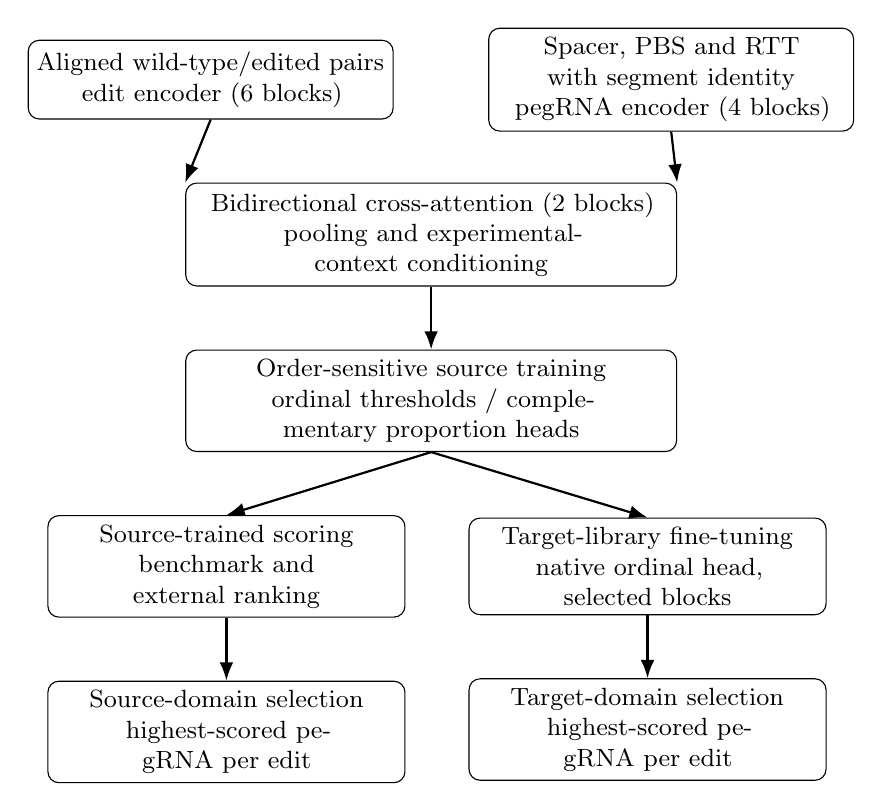
\begin{tikzpicture}[node distance=8mm,box/.style={draw,rounded corners,align=center,text width=4.4cm,minimum height=10mm,font=\small},arr/.style={-{Latex},thick}]
\node[box] (edit) {Aligned wild-type/edited pairs\\edit encoder (6 blocks)};
\node[box,right=12mm of edit] (peg) {Spacer, PBS and RTT with segment identity\\pegRNA encoder (4 blocks)};
\node[box,below=of edit,xshift=2.8cm,text width=6cm] (cross) {Bidirectional cross-attention (2 blocks)\\pooling and experimental-context conditioning};
\node[box,below=of cross,text width=6cm] (source) {Order-sensitive source training\\ordinal thresholds / complementary proportion heads};
\node[box,below=of source,xshift=-2.6cm,text width=4.3cm] (rank) {Source-trained scoring\\benchmark and external ranking};
\node[box,right=8mm of rank,text width=4.3cm] (adapt) {Target-library fine-tuning\\native ordinal head, selected blocks};
\node[box,below=of rank,text width=4.3cm] (selectsource) {Source-domain selection\\highest-scored pegRNA per edit};
\node[box,below=of adapt,text width=4.3cm] (selecttarget) {Target-domain selection\\highest-scored pegRNA per edit};
\draw[arr] (edit.south)--(cross.north west);
\draw[arr] (peg.south)--(cross.north east);
\draw[arr] (cross)--(source);
\draw[arr] (source.south)--(rank.north);
\draw[arr] (source.south)--(adapt.north);
\draw[arr] (rank)--(selectsource);
\draw[arr] (adapt)--(selecttarget);
\end{tikzpicture}
\caption{\textbf{\model{} integrates edit-aware representation learning with pegRNA ranking and selection.} Self-attention or bidirectional S4D mixes tokens within each stream; cross-attention connects guide and target. The source ensemble combines ordinal and proportion-based families. External zero-shot ranking uses the five-fold ordinal--S4D ensemble, whereas target fine-tuning starts from a predetermined single ordinal--S4D checkpoint and retains its native score. These are distinct configurations of the framework. No OptiPrime predictions or parameters enter the model. The supplementary adaptation experiments test additional selector and preservation variants, not required components of the main method.}
\label{fig:architecture}
\end{figure}


\subsection{PE-RankFormer outperforms OptiPrime across source rank-based metrics}
The source corpus comprises 318,471 measurements, with 297,962 training/development rows and 20,509 official held-out rows. The held-out benchmark includes 9,175 Liu-derived and 11,334 Kim-derived measurements.
On the original held-out benchmark, the frozen heterogeneous \model{} ensemble reached \rhoS{} $=0.9079$, compared with $0.8690$ for released OptiPrime (Figure~\ref{fig:prediction}; Table~\ref{tab:source}). The paired difference was $+0.0389$, with the original 5,000-resample protospacer bootstrap interval $[+0.0286,+0.0498]$. The difference was larger in Kim-derived records than in Liu-derived records. Within 14 sufficiently populated source/cell/editor conditions, the row-weighted average correlation was $0.8111$ versus $0.7605$, a difference of $+0.0506$ with interval $[+0.0345,+0.0670]$. The gain therefore does not disappear when between-condition differences are removed.

\begin{table}[htbp]
\centering\small
\caption{PE-RankFormer outperforms OptiPrime across source rank-based metrics.}
\label{tab:source}
\begin{tabular}{lrrr}
\toprule
Endpoint & OptiPrime & \model{} & Difference \\
\midrule
Pooled Spearman, 20,509 rows & 0.8690 & 0.9079 & +0.0389 \\
Liu Spearman, 9,175 rows & 0.8365 & 0.8585 & +0.0220 \\
Kim Spearman, 11,334 rows & 0.7320 & 0.8124 & +0.0803 \\
Within-condition mean Spearman & 0.7605 & 0.8111 & +0.0506 \\
Within-protospacer mean Spearman & 0.5472 & 0.6356 & +0.0884 \\
Kendall's tau-b & 0.6931 & 0.7478 & +0.0547 \\
Positive-outcome Spearman & 0.8256 & 0.8725 & +0.0469 \\
\bottomrule
\end{tabular}
\par\smallskip\begin{minipage}{\linewidth}\footnotesize
Differences are calculated before rounding. Within-protospacer correlation averages 670 eligible groups; these can contain multiple edits and conditions and are not fixed-edit utility. Positive-outcome correlation uses 15,008 rows with nonzero measured editing. Source benchmark numbers are not scores of the later adapted single-checkpoint models.
\end{minipage}
\end{table}

\begin{figure}[htbp]
\centering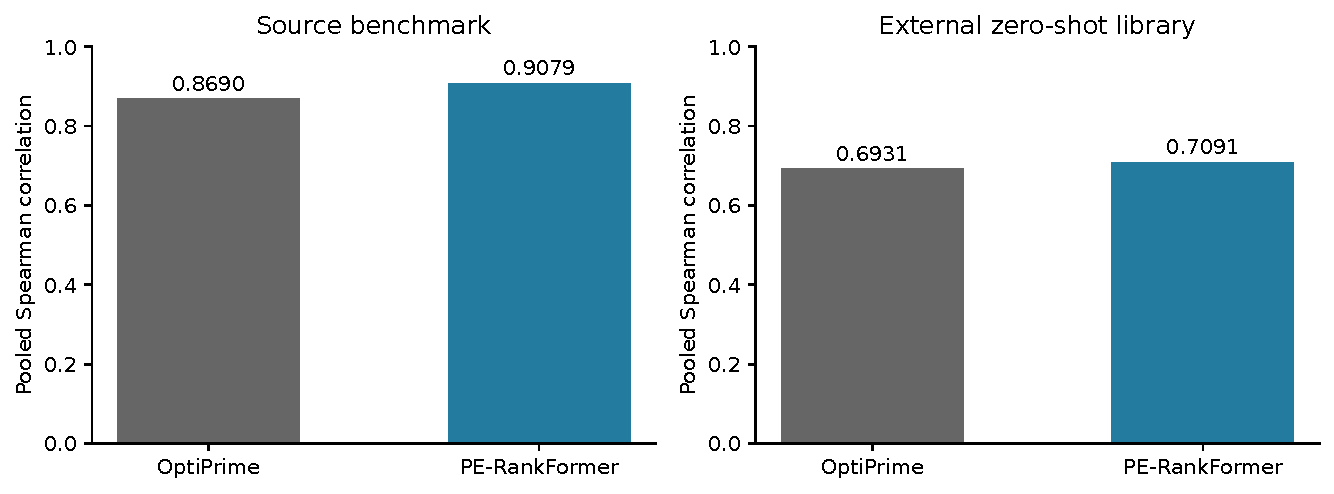
\includegraphics[width=\linewidth]{figures/prediction.pdf}
\caption{\textbf{The ranking advantage extends from the source benchmark to the external library.} Bars show pooled Spearman correlation on the source benchmark and initially reserved external library. The source panel uses the heterogeneous ensemble; the external panel uses its ordinal--S4D member ensembled over five folds. Both comparisons use source-trained models without target-library fine-tuning. Different model configurations and populations preclude interpreting the between-panel change as a controlled estimate of domain shift.}
\label{fig:prediction}
\end{figure}


The ranking advantage also holds within protospacer groups: mean Spearman correlation over 670 eligible groups was $0.6356$ versus $0.5472$, a gain of $0.0884$ (95\% interval $[0.0761,0.1007]$). Because these groups can span edits and conditions, we interpret this as a local ranking endpoint rather than a fixed-edit selection result. Kendall's tau-b increased from $0.6931$ to $0.7478$, with difference $+0.0547$ and interval $[+0.0426,+0.0674]$. Restricting Spearman to positive measured outcomes retained a gain of $+0.0469$ (interval $[+0.0340,+0.0613]$). The improvement therefore extends beyond pooled Spearman and is not explained solely by identifying zero-valued outcomes. Absolute-efficiency calibration and additional robustness checks are reported in Supplementary Sections~\ref{sec:supcalibration} and \ref{sec:suprobust}.

\subsection{The ranking advantage transfers to an external pegRNA library}
We reconstructed the masked edited-sequence representation in the DeepPrime large variant library and removed records sharing the audited protospacer or canonical allele with the source corpus. The resulting panel contains 118,187 measurement rows, corresponding to 118,174 distinct candidates in 30,475 eligible decisions. Unlike the source decision subset, it contains 8,775 groups with at least five candidates and 2,400 with at least eight. Its outcome distribution and PBS/RTT geometry also differ from those of the source benchmark. The initial panel endpoints, grouping and eligibility were declared locally before the original model scoring.


Without target-library training, the ordinal--S4D ensemble achieved pooled Spearman correlation $0.7091$, compared with $0.6931$ for OptiPrime (Figure~\ref{fig:prediction}). This transfer result extends the rank-based advantage beyond the source benchmark, despite changes in candidate depth, PBS/RTT geometry and measured outcome distribution. The external library is a distinct panel from a study also represented in source training; overlap exclusion does not make it an independent-study holdout.

\subsection{Improved source ranking is accompanied by higher top-choice selection efficiency}
We next asked whether improved ranking translates into better pegRNA selection for a fixed intended edit. Canonicalization of the full corpus yielded 51,766 intended alleles and 175,668 allele/context decision groups. The source evaluation fold contains 2,412 groups with at least two distinct candidates, only 85 with at least three, and none with five. Among these, 1,463 groups have nonconstant measured outcomes and support an informative choice. A conventional protospacer grouping instead pools alternatives across conditions and sometimes across desired alleles. We retain within-protospacer correlation as a descriptive statistic, but do not substitute it for the fixed-edit decision endpoint.

On the informative source decisions, the heterogeneous ensemble's top-choice efficiency was $0.13636$ versus $0.12721$ for OptiPrime, a paired gain of $0.00915$ (95\% interval $[0.00633,0.01215]$). Its measured-best-design hit rate was $0.7423$ versus $0.6535$, and regret was $0.00667$ versus $0.01582$. The efficiency gain is a 7.2\% relative improvement, accompanied by an 8.89-percentage-point increase in measured-best-design hit rate. Thus, \model{} improves both overall ordering and the outcome of selecting a single candidate in the source domain. These decisions are predominantly shallow and Kim-derived; they do not establish the same benefit for deeper external candidate sets (Supplementary Table~\ref{tab:decision}).


\subsection{Target-library fine-tuning enables an external selection advantage over OptiPrime}
Native-ordinal fine-tuning provides a second selection-efficiency result, now on the external library (Figure~\ref{fig:selection}; Table~\ref{tab:ordinalselection}).
We next partitioned external-library locus components into adaptation training, validation and test roles. Full-budget fitting used 19,357 training groups, and checkpoint selection used 5,561 validation groups. The retrospective test subset comprised 5,557 groups and 23,044 candidates. The test role prevented direct checkpoint selection on those rows, but this was a repartition of an already studied library, not a new independent study.

Ordinary native-ordinal adaptation achieved mean test utility $0.04178$ over three optimizer seeds, compared with $0.04020$ for released OptiPrime (Table~\ref{tab:ordinalselection}). The gain, approximately $0.00158$ or $0.158$ percentage points of editing efficiency, corresponds to a 3.9\% relative increase and about a 15.7\% reduction in measured oracle regret. Each ordinal seed's paired component interval against OptiPrime was positive. Pooled test Spearman was $0.7771$ versus $0.6922$. This establishes a benefit for target-supervised \model{} relative to the unadapted released comparator, not superiority under equal target-label access.


\begin{table}[htbp]
\centering\small
\caption{Native-ordinal fine-tuning improves external selection over released OptiPrime.}
\label{tab:ordinalselection}
\begin{tabular}{lrrr}
\toprule
Optimizer seed & \model{} $U_1$ & $\Delta$ OptiPrime & Paired 95\% interval \\
\midrule
20260910 & 0.04182 & +0.00162 & $[+0.00094, +0.00227]$ \\
20260911 & 0.04174 & +0.00154 & $[+0.00086, +0.00218]$ \\
20260912 & 0.04178 & +0.00157 & $[+0.00091, +0.00223]$ \\
\bottomrule
\end{tabular}
\par\smallskip
\begin{minipage}{\linewidth}\footnotesize Same retrospective E25 test for every row: 5,557 groups, 23,044 candidates and 4,954 locus components. OptiPrime top-choice efficiency is 0.04020; the mean adapted outcome across seeds is 0.04178. Intervals resample paired locus components conditional on each fitted model, not training seeds or independent studies. All entries are efficiency fractions. Adaptation uses 19,357 training and 5,561 validation groups; OptiPrime receives no target labels.\end{minipage}
\end{table}


\begin{figure}[htbp]
\centering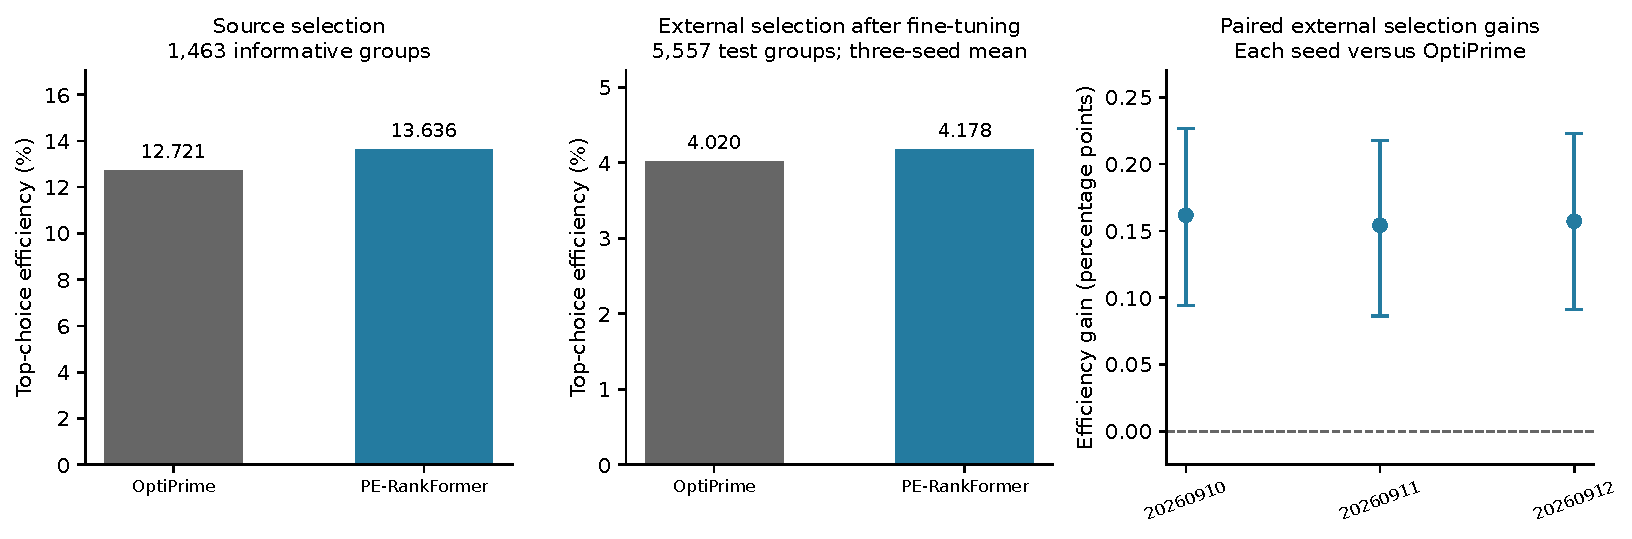
\includegraphics[width=\linewidth]{figures/selection.pdf}
\caption{\textbf{\model{} improves selection in the source domain and after target-library fine-tuning.} Left: source top-choice efficiency over 1,463 informative fixed-edit groups, using the frozen heterogeneous ensemble. Center: retrospective external test efficiency over 5,557 groups, using native-ordinal adaptation (mean outcome across three optimizer seeds). Right: each adapted seed's paired efficiency gain over OptiPrime with its 95\% locus-component bootstrap interval; zero denotes equal top-choice efficiency. The seed intervals condition on the fitted models and are not independent-study replications. The external models use 19,357 training and 5,561 validation groups; released OptiPrime is unadapted. Source and external panels use different populations and model configurations, so their absolute heights are not a paired domain-shift comparison.}
\label{fig:selection}
\end{figure}

Target supervision is an essential condition of the demonstrated external selection advantage. Before fine-tuning, the source-trained ordinal--S4D ensemble's external top-choice efficiency was $0.03627$ versus $0.03690$ for OptiPrime, a difference of $-0.00064$ (95\% interval $[-0.00089,-0.00038]$) on the full 30,475-group panel. Its higher pooled correlation therefore did not by itself guarantee better within-edit selection. Fine-tuned and zero-shot numbers above are evaluated on different denominators; the adaptation result is established by comparing methods on the same 5,557-group test subset, not by subtracting their full-panel and test-subset means. Detailed zero-shot depth-stratified comparisons remain in Supplementary Section~\ref{sec:suptransfer}.

\subsection{Controlled extensions define the supported model and adaptation regime}
Development comparisons support ordinal supervision and S4D within the framework: the retrospective average objective and mixer contrasts in source out-of-fold Spearman were $+0.0092$ and $+0.0192$, respectively. These comparisons are observational rather than a fully matched factorial. Source weighting, ensemble composition and canonical batching also affect results, preventing attribution of the entire OptiPrime margin to one component (Supplementary Sections~\ref{sec:supmodelcontrols} and \ref{sec:supgroupcontrols}).

The native-ordinal fine-tuning result does not depend on a more complex selection head. Separate utility and multitask heads did not establish a replicated additional target advantage, and apparent source retention could disappear when evaluated using their deployed selector instead of an unused prediction head (Supplementary Section~\ref{sec:supheadcontrols}). We therefore emphasize native-ordinal adaptation as the supported procedure for the full-budget selection comparison.

More stringent low-label and source-retention requirements remain unresolved. In the acquisition-replicated, nominal 1,000-group study, neither tuned ordinal adaptation nor source anchoring established a selection win over OptiPrime. A balanced teacher-margin constraint improved retention relative to unconstrained anchoring but sacrificed target utility when source constraints governed checkpoint selection. These results involve an exposed outer development subset and a different label budget, not a refutation or independent confirmation of the full-budget test result (Supplementary Sections~\ref{sec:suplowlabel} and \ref{sec:supretention}). No additional independent-study model evaluation was completed (Supplementary Section~\ref{sec:supdeployment}).
\FloatBarrier

\section{Discussion}
\model{} advances pegRNA ranking through edit-aware sequence modeling and order-sensitive supervision. Relative to released OptiPrime, its source ensemble improves pooled Spearman correlation, correlation within experimental conditions, correlation within protospacer groups and Kendall's tau-b. A positive-outcome-only analysis retains the advantage, and the ordinal--S4D ensemble extends higher pooled correlation to an external library. Together, these results show that the source ranking gain is not confined to a single metric, one source-study subset or the separation of zero from nonzero outcomes.

The architecture provides a coherent way to represent the design problem. Aligned wild-type/edited pairs expose the intended change, segment-aware pegRNA encoding distinguishes functional sequence regions, and cross-attention integrates guide and target information. Context conditioning supports a heterogeneous training corpus. Ordinal supervision supplies multiple outcome-threshold comparisons rather than requiring the ranking score itself to be a calibrated efficiency. The development comparisons support ordinal supervision and S4D as useful choices within this framework. They do not isolate a uniquely causal component: the historical comparisons are not a fully matched randomized factorial, and the systems also differ in training weights and ensemble composition. We accordingly attribute the benchmark improvement to the evaluated \model{} system, not exclusively to one architectural mechanism.

Importantly, the contribution extends beyond correlation. On informative source decisions, \model{} increases the measured efficiency of the selected pegRNA by 7.2\% relative to OptiPrime and raises the measured-best-design hit rate from 65.35\% to 74.23\%. Target-library fine-tuning then establishes an external selection advantage: native-ordinal adaptation improves mean top-choice efficiency by 3.9\% relative to released OptiPrime, with positive paired intervals in all three optimizer seeds. Ordinary ordinal adaptation is sufficient for this result; separate utility or multitask heads do not establish a replicated additional advantage over it. These findings favor a simple supported adaptation procedure over treating an unvalidated extra branch as an essential part of the method.

The external results also define when this selection claim applies. The source-trained ordinal--S4D ensemble has higher external pooled correlation but lower zero-shot top-choice efficiency than OptiPrime. Ranking across a library and ordering alternatives within a fixed edit emphasize different variations, particularly when candidate depth, sequence geometry and outcome distributions change. Fine-tuning demonstrates that target supervision can improve the relevant choices, but does not by itself identify which aspect of domain shift caused the zero-shot shortfall. Nor does it establish that ranking-specific losses are necessary: accurate conditional-mean estimates would also suffice for expected-efficiency selection. Our evidence supports a source-trained ranking advantage and a target-supervised selection advantage, not unconditional superiority on every deployment endpoint.

Label availability and source retention remain practical constraints. In the budget-accounted follow-up, adequately tuned ordinal adaptation and a source-anchored selector did not establish better external selection than OptiPrime at a nominal 1,000-group budget. Balanced teacher-margin preservation improved source retention relative to unregularized anchoring, but source-constrained checkpoint selection incurred a target-efficiency cost. These supplementary results concern additional low-label and retention requirements; they do not negate the full-budget adaptation result, nor justify extending it to lower budgets. Auditing the score actually used to select candidates was essential, because an unchanged prediction head could conceal forgetting in a separate deployed selector.

Several qualifications delimit the comparisons. The source benchmark was revisited during model development and subsequent audits. The external library was initially reserved, but later reused extensively; even the full-budget adaptation test is a retrospective within-library evaluation rather than a new independent study. Moreover, OptiPrime did not receive the target labels used for \model{} fine-tuning. The external selection win is therefore a practical comparison with a released tool, not an equal-label comparison of adaptation methods. The source selection population is shallow and Kim-derived, while pooled ranking also includes Liu-derived records. Repeated optimizer seeds quantify one form of training variability, not generalization across laboratories or studies. Measured maxima contain assay noise and are not noise-free biological optima. Our claims concern the stated populations and released comparator, not every application of OptiPrime \citep{hsu2026}.

Reproducible deployment also requires explicit model identity. The heterogeneous source ensemble, five-fold ordinal--S4D transfer ensemble and fine-tuned single backbone are different configurations of the framework. Population-rank averaging in the historical source ensemble requires a fixed reference transformation or a validated alternative interface for isolated queries. Legacy RNA/DNA tokenization must be handled consistently. The harmonized corpus includes author-supplied material with unresolved redistribution permissions, and the recorded inference timings do not establish a speed advantage over OptiPrime. The accompanying aggregate evidence, buildable manuscript and deployment audits document these boundaries without substituting for a complete public-data release.

The next computational confirmation should freeze the supported ordinal adaptation procedure, account for both training and validation labels, and evaluate ranking and deployed top-choice efficiency on verified independent fixed-edit decisions. An equal-target-label comparator and a source-training study holdout would address fairness and cross-study transfer separately. Higher-label learning curves and carefully controlled representation changes could then determine how far the external selection advantage extends. These are future tests, not completed evidence.

In conclusion, \model{} is a new pegRNA-ranking framework that outperforms released OptiPrime across the evaluated source rank-based metrics and retains higher pooled ranking accuracy on an external library. Its ranking gains translate into improved source-domain guide selection, and native-ordinal fine-tuning enables an additional external-library selection-efficiency advantage. These are the central contributions of the method; the accompanying controls establish the conditions under which each is supported.

\section{Methods}
\subsection{Study design and data provenance}
This is a retrospective computational study of previously measured prime-editing outcomes. No new biological experiments, patient recruitment or interventions were performed. The source corpus is the exact harmonized training/evaluation mixture supplied by the OptiPrime authors, comprising 58 input tables and 318,471 rows. The 297,962 figure refers to training/development rows, not the combined dataset. In particular, the 9,175 Liu-derived held-out measurements must not be removed through an inferred quality-control filter. Source-study identifiers follow the repository conventions \texttt{deepprime}, \texttt{hsu2026} and \texttt{pridict\_pridict2}; these denote harmonized sources rather than claims of uniform assay conditions within each study.

Outcome values are editing-efficiency fractions in $[0,1]$. Indel measurements are absent for approximately 42.5\% of source rows and are not imputed as measured zeros. Approximately 16.0\% of training efficiencies are exactly zero; the corresponding proportions on source held-out and matched development populations are 26.8\% and 28.4\%. These are measurement properties, not proof that the latent editing probability is zero. The source files, processed-table hashes and reconstruction scripts are indexed in the accompanying evidence inventory.

We preserve the official five development folds and held-out fold zero. Later matched development populations were sampled at the protospacer level to approximate the Liu/Kim evaluation mixture, with overlapping source identifiers handled by the documented exclusions. Every development-row ensemble prediction uses only its official-fold-held-out checkpoint, rather than averaging checkpoints that trained on that row. For genuinely external and fold-zero rows, all five checkpoints in a family can contribute. The historical internal gate comprises 17,975 rows and 367 protospacers disjoint from the matched development validation populations. It was nevertheless used to choose between shortlisted models, and is described as a selection gate rather than a wholly unused confirmatory test.

\subsection{Canonical intended alleles, candidate identity and dependence}
An intended edit is identified from its wild-type and edited target sequences, normalizing equivalent representations in repeated sequence and reconciling strand orientation. The corrected canonicalizer independently normalizes the forward and reverse-complement orientations before selecting a canonical representation. Reverse-complementing an already left-normalized indel alone is insufficient because each orientation has its own leftmost representation. This operation canonicalizes allele identity; it is not label-preserving augmentation of pegRNA molecules.

A decision group fixes this intended allele and its experimental context, including the applicable cell/editor and construct metadata. A candidate is a distinct design in that group, not an individual measurement row. Repeated measurements for the same group/design are averaged before decision ranking; the number of contributing records is retained. This collapses thirteen external rows without reducing the 30,475 eligible group count. Prediction-level analyses that explicitly use measurement rows retain their original row denominator. Outcome-defined informative groups have at least two distinct candidates and nonconstant outcomes; primary target-adaptation and external-all analyses retain all eligible groups, including all-zero groups.

The early source uncertainty analyses resample protospacers; corrected source decision analyses contain 439 such clusters. Later adaptation joins canonical alleles and protospacers into connected locus components for splitting and resampling, because an allele can be reached by several protospacers and a protospacer can install several alleles. The same 1,463 informative source-audit groups then form 437 connected components. These informative source decisions are Kim-derived; pooled source prediction metrics also include Liu-derived records. The E25 target-validation and test sets contain 4,952 and 4,954 components, respectively. These dependence definitions are recorded alongside the corresponding estimates rather than treated as interchangeable.

\subsection{External-library reconstruction and overlap checks}
The external library derives from the large DeepPrime variant dataset \citep{yu2023}, not the LibSmall files included in the harmonized source mix. Its released edited-target field is masked outside the RT/PBS footprint. Reconstruction uses the supplied wild-type sequence, edit annotations and PBS/RTT frame, with orientation and nick-position checks. The recorded checks include agreement on all 153,974 substitution rows for the nick-position relation and cross-checks of reconstructed PBS/RTT strings against matching source records. Eligibility and canonical grouping were fixed before the initial model scoring, with input fingerprints retained.

The initial panel removes overlap under the declared protospacer/allele rules. Later audits additionally normalize RNA/DNA alphabets, compare spacer cores and inspect local homology. The final shared-core sensitivity excludes an entire affected component, not just the matching candidate. These checks reduce identifiable overlap but do not prove complete absence of all biological or evolutionary dependence. Released DeepPrime is not a clean held-out comparator on a library used in its own training; we therefore do not report its released score as an independent benchmark here. Separate PRIDICT/DeepPrime reproduction attempts were not completed and are not presented as negative performance results.

\subsection{Sequence architecture}
The edit stream represents aligned wild-type/edited base pairs, capped at 100 paired positions plus sentinels. The pegRNA stream represents a nucleotide sequence assembled in spacer/PBS/RTT order, capped at 90 total positions including sentinels (at most 88 nucleotides), with learned functional-segment embeddings. The actual RNA/string convention follows the frozen preprocessing implementation. Positional and segment information expose geometry in principle, although accessibility to a learned readout is an empirical issue.

The base network has six edit-encoder blocks, four pegRNA-encoder blocks and two bidirectional cross-attention blocks, width 384, six attention heads, feed-forward width 1,536 and dropout 0.1. Attention follows the multi-head formulation of \citet{vaswani2017}. Attention-pooled stream representations are combined with experimental context. Cell type, editor system, Cas9 variant, PAM, scaffold, 3-prime motif and source are categorical inputs. Feature-wise linear modulation applies
\begin{equation}
 h'=\{1+\gamma(c)\}\odot h+\beta(c),
\end{equation}
where the context vector $c$ is mapped to channel-wise scale and shift \citep{perez2018}. Some model families apply conditioning at each block rather than only near the readout. Architecture variants have approximately 25 million parameters; a subset includes an explicit engineered-feature branch. We do not characterize the full heterogeneous ensemble as feature-free.

\begin{figure}[htbp]
\centering
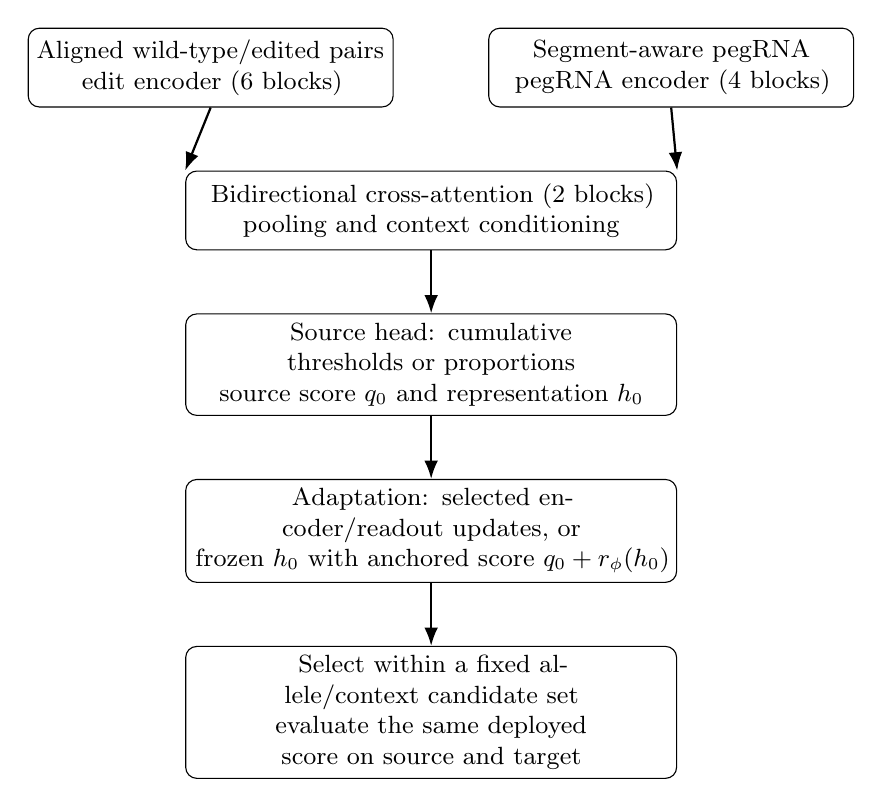
\begin{tikzpicture}[node distance=8mm,box/.style={draw,rounded corners,align=center,text width=4.4cm,minimum height=10mm,font=\small},arr/.style={-{Latex},thick}]
\node[box] (edit) {Aligned wild-type/edited pairs\\edit encoder (6 blocks)};
\node[box,right=12mm of edit] (peg) {Segment-aware pegRNA\\pegRNA encoder (4 blocks)};
\node[box,below=of edit,xshift=2.8cm,text width=6cm] (cross) {Bidirectional cross-attention (2 blocks)\\pooling and context conditioning};
\node[box,below=of cross,text width=6cm] (source) {Source head: cumulative thresholds or proportions\\source score $q_0$ and representation $h_0$};
\node[box,below=of source,text width=6cm] (adapt) {Adaptation: selected encoder/readout updates, or\\frozen $h_0$ with anchored score $q_0+r_\phi(h_0)$};
\node[box,below=of adapt,text width=6cm] (select) {Select within a fixed allele/context candidate set\\evaluate the same deployed score on source and target};
\draw[arr] (edit.south)--(cross.north west);
\draw[arr] (peg.south)--(cross.north east);
\draw[arr] (cross)--(source);\draw[arr] (source)--(adapt);\draw[arr] (adapt)--(select);
\end{tikzpicture}
\caption{\textbf{Sequence prediction and deployed-score adaptation.} Encoder blocks use self-attention or bidirectional S4D according to the model family. The anchored readout uses a training-standardized source score (normalization omitted from the diagram). Historical heterogeneous ensembling and the single-backbone adaptation procedures are distinct deployments. No comparator predictions enter the adaptation path.}
\label{fig:architecture}
\end{figure}

S4D replaces the within-stream attention mixer with a diagonal state-space convolution \citep{gu2022s4d}; cross-attention remains. For diagonal state matrix $A$, discretization step $\Delta$ and output coefficients $C$, a kernel can be written as
\begin{equation}
K[\ell]=2\operatorname{Re}\sum_n C_n\frac{\exp(\Delta A_n)-1}{A_n}\exp(\ell\Delta A_n).
\end{equation}
Independent forward and reversed kernels provide bidirectional mixing, implemented with FFT convolution and padding masks. The tested state dimension is 64. These short sequence lengths and our implementation-specific controls do not support general computational superiority of state-space models over attention.

\subsection{Source objectives, optimization and ensembling}
The cumulative-threshold head uses de-duplicated quantiles $t_1<\cdots<t_J$ estimated only from the corresponding training rows. Independent logits $z_j(x)$ are trained by
\begin{equation}
\mathcal L_{\rm ord}(x,y)=\frac1J\sum_{j=1}^J\operatorname{BCEWithLogits}\left(z_j(x),\mathbf1\{y>t_j\}\right),\qquad
q(x)=\frac1J\sum_{j=1}^J\sigma(z_j(x)).
\label{eq:ordinal}
\end{equation}
Nominally twenty quantile levels yield seventeen distinct thresholds in the twenty audited official-fold ordinal checkpoints (including candidate families outside the final ensemble) and eighteen in the matched development-fold models. This target transformation encourages order-sensitive prediction but is not a direct optimization of sample Spearman or a proof of Fisher consistency for the deployment endpoint. Unlike a rank-consistent parameterization \citep{cao2020}, independent threshold logits need not be monotone across thresholds. Shared-parameter and monotonicity-penalty controls were tested separately.

The simplex head predicts three softmax channels and uses soft cross-entropy for observed unedited, correctly edited and indel fractions, after clipping/renormalization in the implementation. When indel is missing, the implementation instead normalizes the first two logits and trains against $(1-y,y)$. We describe this precisely as a two-class fallback: without assumptions about the assay denominator, it is not automatically the exact marginal likelihood of an unobserved indel fraction. Its ranking score is $z_E-z_U$. Scalar Huber, auxiliary losses and additional head variants are catalogued in the supplement.

The standard source recipe uses AdamW, learning rate $3\times10^{-4}$, weight decay 0.01, five-percent linear warmup followed by cosine decay, gradient clipping at norm one, batch size 512, BF16 mixed precision and a thirty-epoch budget. Validation Spearman chooses the checkpoint; patience equals the maximum epoch budget. Run configurations record departures from this base recipe. Group-aware batching supports optional ranking losses. Because the historical group key affects both batching and pair eligibility, changing it is not a pure objective intervention; the later arm matrix explicitly separates these factors.

The final source ensemble includes ordinal--S4D, simplex--S4D, ordinal Transformer with layerwise FiLM, ordinal Transformer with a feature branch, and simplex Transformer with layerwise FiLM. The feature branch receives sixteen implemented scalar inputs: PBS/RTT lengths, PBS/RTT/extension GC fractions, edit length, edit position, edit position from the nick, mismatch count, PBS/RTT melting temperatures, four folding-energy features and RuleSet3 activity. Missingness indicators accompany training-standardized features. The corpus and source family configuration are fixed; this feature set is not selected on external outcomes.

For source ensemble inference, each family's external predictions are averaged across its five fold checkpoints, converted to fractional ranks over the evaluation population, and equally averaged across the five selected families. Rank averaging is population-dependent; production use on isolated queries would require an explicitly fixed reference transformation or a validated alternative scoring interface. We do not assume arbitrary inference batching reproduces this ensemble. For development, each row contributes only an out-of-fold checkpoint prediction. Later adapted models use a directly deployable individual score rather than this population-rank ensemble.

Isotonic regression maps source-development out-of-fold rank scores to efficiencies and is transferred without fitting to the evaluated outcomes. This is a nondecreasing map, which cannot reverse ordered pairs but may collapse distinctions into ties, especially with out-of-range clipping. We report raw-score rankings and calibrated absolute-error endpoints separately. Absolute calibration on a shifted study requires its own validation.

\subsection{Decision endpoints}
For group $g$, let $n_g$ denote distinct candidates, $y_{gi}$ their aggregated measured efficiencies, and $s_{gi}$ their deployed scores. Let $\pi_g$ sort candidates by decreasing score, breaking score ties deterministically by the stored canonical design order. For $\mathcal G_k=\{g:n_g\geq\max(2,k)\}$, define
\begin{align}
U_k(s)&=\frac{1}{|\mathcal G_k|}\sum_{g\in\mathcal G_k}\max_{1\leq j\leq k}y_{g,\pi_g(j)},\\
R_1(s)&=\frac{1}{|\mathcal G_1|}\sum_g\left[\max_i y_{gi}-y_{g,\pi_g(1)}\right],\\
H_1(s)&=\frac{1}{|\mathcal G_1|}\sum_g\mathbf1\{y_{g,\pi_g(1)}=\max_i y_{gi}\}.
\end{align}
All group means weight decisions equally rather than weighting by candidate count. Informative-only endpoints restrict the population explicitly. The oracle is the mean measured maximum on the same population; it is a retrospective upper reference, not an estimate of noise-free biological optimality. The random hit baseline credits every tied maximizer, including all candidates in an all-zero group. For ordered outcomes $y_{g(1)}\leq\cdots\leq y_{g(n)}$, random top-$k$ utility is computed exactly as
\begin{equation}
\mathbb E[U_{k,g}^{\rm random}]=\sum_{i=k}^{n}y_{g(i)}\frac{\binom{i-1}{k-1}}{\binom{n}{k}}.
\end{equation}
Top-$k$ denotes the best measured outcome among the nominated $k$, not the average nominated outcome. Groups with insufficient depth are undefined for that endpoint rather than silently truncated. Depth-conditioned curves must use their stated population-specific oracle and random references.

\subsection{Historical target-supervised adaptation}
All adaptation begins from the predetermined official-fold-one ordinal--S4D checkpoint, not the best checkpoint selected on external outcomes. Historical ordinal P updates the original head, pooling, context FiLM, cross-attention and final edit/pegRNA encoder blocks. Utility S adds a scalar selector and trains for selection; multitask M jointly trains original prediction and selection losses; frozen Z updates only the new head. A shared-score control allocates extra capacity without separate deployed scores. These historical letters are local experiment labels: historical multitask M is not the later margin-preservation M.

The historical budget is twelve epochs with patience four, whole-group batches capped at 512 candidates, AdamW with weight decay 0.01, effective base learning rate $3\times10^{-5}$ and new-head learning rate $10^{-3}$. Computation uses BF16. The initial loss magnitudes are measured on up to twelve training batches to set fixed normalization constants; this normalization does not match gradient magnitudes or score scale across objectives. Checkpoints maximize validation top-choice utility. Historical runs using 200, 1,000 or 5,000 \emph{training} groups still use all 5,561 validation groups and are not total-label-budget experiments.

Selection-only and multitask variants use a soft expected-regret loss,
\begin{equation}
\mathcal L_{\rm util,g}=\frac{\max_i y_{gi}-\sum_i p_{gi}y_{gi}}{a},\qquad
p_{gi}=\frac{\exp(s_{gi}/T)}{\sum_j\exp(s_{gj}/T)},
\label{eq:util}
\end{equation}
with fixed training-derived normalization $a$, $T=1$ and constant-outcome groups omitted from the selection-gradient average. A listwise alternative uses cross-entropy against $\operatorname{softmax}(y/0.02)$. Pairwise training weights logistic errors by $w_{ij}=\min(|y_i-y_j|,0.05)$ and normalizes by the sum of weights within a group. Historical pairwise runs sample at most eight pairs per group; later low-label runs use all within-group pairs. No positive minimum-gap threshold is imposed in these adaptation losses. All methods deploy deterministic argmax scores, not stochastic softmax samples.

\subsection{Budget-accounted anchored adaptation}
Low-label experiments reserve inner validation within each acquired set of entire locus components. Per-fit target-training score means and standard deviations are computed without inner or outer labels. With frozen representation $h_0$ and source score $q_0$, anchored adaptation uses
\begin{equation}
s_\phi(x)=\frac{q_0(x)-\mu_{q,\rm train}}{\sigma_{q,\rm train}}+r_\phi(h_0(x)).
\end{equation}
The residual network has layer normalization, a 768-to-256 linear layer, GELU, dropout 0.1 and a scalar projection, totaling 198,657 trainable parameters. Zero-initializing the final projection reproduces the original ordering before training. Fresh frozen controls have the same readout form without the residual source score. Ordinal and shared-regression controls update the same final-block/readout modules as the historical ordinary-adaptation baseline. The fresh selector therefore has fewer trainable parameters, but deployment still requires the approximately 24.88-million-parameter pretrained encoder/readout system; it is not a 198,657-parameter standalone predictor.

The initial low-label study fixes 100 target updates, whole groups, a 256-candidate cap, clipping at one, FP32 with TF32 disabled, base learning rate $3\times10^{-5}$ and selector learning rate $10^{-3}$. The follow-up controls cross multipliers one and three with 100 and 500 updates for five arms: native ordinal, standardized Huber regression, shared Huber-plus-pairwise score, fresh frozen pairwise and anchored frozen pairwise. Different horizons and active modules imply different data passes and compute; update counts are not a claim of equal FLOPs. The selected ordinal recipe uses 100 updates and multiplier three; the selected anchored recipe uses 100 updates and multiplier one. Each configuration is selected by its budget-inner outcome, never by promoting the best outer-audit score.

Step zero and ten equally spaced checkpoints are evaluated. Target-only selection maximizes inner $U_1$, preferring the earliest checkpoint within $10^{-12}$ ties. Source-constrained selection first requires each eligible source-validation study's point loss relative to initialization to be no greater than 0.001, then maximizes inner target utility. Initialization is always eligible, including for procedures with freshly initialized heads, so failure to find a feasible adaptation produces a genuine no-adaptation fallback. This policy is an operational filter, not a statistical noninferiority certificate.

\subsection{Source preservation and replication}
Replay and retention-validation components exclude source fold zero and connections to target-panel alleles/protospacers under the recorded construction. Both replay and source-validation rows were available during source pretraining. The informative replay pool comprises 486 DeepPrime and 2,461 PRIDICT-family groups; source validation comprises 72 and 613 groups, respectively. Liu-derived singleton groups do not enter the selection-preservation objective. The source audit is distinct from replay and checkpoint selection but has informed research direction.

Soft preservation averages Bernoulli KL between teacher and adapted score-difference probabilities over within-group pairs. Teacher-margin preservation instead identifies the teacher's deterministic winner $b_g$ and uses
\begin{equation}
\mathcal L_{\rm margin,g}=\frac{1}{n_g-1}\sum_{j\neq b_g}
\left[\min\{q_{0,b_g}-q_{0,j},c\}-(s_{b_g}-s_j)\right]_+,
\label{eq:margin}
\end{equation}
where $q_0$ denotes the training-standardized teacher score, and $c$ is the ninetieth percentile of teacher-winner gaps on source training. There is no positive floor for teacher ties. A measured-source utility loss uses Equation~\ref{eq:util}, normalized by the training-pool mean positive outcome range. These constraints preserve our source model or source labels, not comparator behavior.

The twelve-run factorial crosses the three source objectives, source-mixture versus equal-study sampling, and weights 0.1 versus 1. Groups are sampled with replacement across updates but without duplicate groups inside a batch, subject to a 256-candidate cap. Group indivisibility means candidate counts are not exactly matched; realized source exposure and weighted-source/target gradient ratios are recorded. A maximum of one recipe is promoted by constrained inner utility, requiring an improvement of at least 0.0005 over constrained anchoring. This selects balanced teacher-margin weight one. The selection rule was recorded locally before its stage, not publicly registered.

Locked replication uses acquisition seeds 20260910, 20260911 and 20260912 and two optimizer seeds per acquisition, at nominal 200- and 1,000-group budgets. Four methods produce 48 configurations; four exact screen fits are reused, so forty-four additional fits complete replication and the follow-up total is 76, not 80. The union of target labels used across these acquisitions is 2,853 groups, 10,507 candidates and 10,508 measurement records, separate from the 23,120 outer-validation candidates and source labels. Higher-label replication, final-block anchored variants, genuinely separate representation branches, and excluded-domain pretraining were not executed.

\subsection{Uncertainty, multiplicity and evaluation exposure}
We use paired percentile bootstraps with the same sampled clusters for both methods. The original source headline uses 5,000 protospacer resamples; corrected fixed-edit endpoints and adaptation use 2,000 site/component resamples. The historical quartet decomposition uses 400 locus resamples. Each estimate is tied to its original ledger and resampling unit. The source prediction benchmark has 750 protospacer clusters; clusters are not independent rows. For replicated adaptation, we first average per-group outcomes over paired fitted runs and then resample evaluation components. These intervals condition on those fitted models and acquisitions. Run standard deviations and acquisition-specific results describe additional observed instability but do not convert the intervals into population-level uncertainty over arbitrary acquisitions or future studies.

The manuscript emphasizes effect sizes and intervals rather than zero bootstrap $p$-values. Empirical tail probabilities are limited by the number of resamples, and a self-comparison must be marked degenerate rather than declared significant. Recorded floating-point discrepancies below $10^{-17}$ in repeated fallback means are treated as numerical identity, not biological evidence. Reported exploratory intervals are not multiplicity-adjusted. Extensive search and retrospective contrasts preclude interpreting nominal 95\% intervals as family-wise or post-selection guarantees. The historical approximately 0.005 development threshold was an operational promotion heuristic based on sign instability, not a universal power bound.

The original held-out benchmark was inspected for four successive model generations and subsequently audited. Pairing controls comparison variance but does not cancel model-specific adaptive selection bias. The external panel's original zero-shot analysis was locally declared before first scoring; later corrective training and adaptation reused its outcomes. Repartitioning this library does not reset that exposure. Budget-inner checkpoint selection keeps individual fits within their declared label budget, but outer results have informed the research program and consume additional outcome information. We therefore distinguish original reserved evaluation, exposed audit, within-budget validation and independent confirmation throughout.

\subsection{Replicate diagnostics and implementation verification}
The source repeatability analysis requires matching all sixteen audited design/context covariates and the target site, yielding 649 strict replicate groups. Broader keys merge distinct constructs and cannot estimate technical repeatability. Empirical nearest-neighbor resampling of 1,298 ordered replicate measurements represents bounded, heteroscedastic outcomes and zero/nonzero discordance. The resulting extrapolated rank-repeatability reference is conditional on representativeness and the resampling model; it is not an identified Bayes-optimal ceiling. The familiar square-root reliability relation additionally requires assumptions about independent measurement error and the correlation scale, and should not be treated as an exact Spearman theorem.

Historical code, model inputs, split manifests, predictions and selected checkpoints have stored fingerprints. The completed follow-up verifies 32 screen fits and 48 replication configurations, including four reused fits: 456 screen fingerprints and 288 endpoints, plus 685 replication fingerprints, 1,056 checkpoint/surface reconstructions and 432 selected/final endpoints. The archived protocol/endpoint suite contains 43 passing tests. These verify the recorded implementation and arithmetic, not independence of the biological evidence. The new manuscript package additionally regenerates aggregate tables and figures without access to private sequence-bearing data. The 76-fit follow-up consumed 2.273 summed process-hours including evaluation and I/O, not pure accelerator kernel-hours or total research-program cost.

\section*{Data availability}
The original biological measurements derive from the cited source studies and their supplementary resources. The exact 318,471-row harmonized corpus was supplied by the OptiPrime authors and includes inputs not fully reconstructed from the public releases. This submission package contains aggregate source data and analysis provenance, not private sequence-bearing tables, acquired raw reads or model checkpoints. Redistribution permission and the final mechanism for qualified access to the complete corpus and checkpoints must be confirmed before submission; no unrestricted release is asserted here. Public-panel accession and reconstruction details are indexed in the repository's data audits.

\section*{Code availability}
The analysis repository is \url{https://github.com/xhxuciedu/PEFormer}. The research state reviewed for this manuscript is commit \texttt{b55a14462a4b7e217041ffd763e90edf83f8860e}; the new manuscript files are a subsequent working-tree addition, not part of that commit. The package contains LaTeX sources, generated aggregate tables, vector figures, a source-data ledger and reproduction/verification instructions. Repository accessibility, the software/checkpoint license and an immutable release archive identifier require confirmation before submission. No archival DOI is claimed.

\section*{Author contributions, funding and competing interests}
\textit{Author-supplied metadata required before submission:} author names, affiliations, corresponding author, contributor roles, funding/support and competing-interest declarations. These statements cannot be inferred from the repository and have not been fabricated. The final manuscript must also contain any applicable disclosure of computational writing or coding assistance under the selected journal's policy.

\section*{Acknowledgements}
The exact harmonized source corpus was made available by the OptiPrime authors. The final acknowledgements and permission to name individuals should be confirmed by the submitting authors.

\begingroup\small
\bibliographystyle{plainnat}
\bibliography{references}
\endgroup
\clearpage
\appendix
\renewcommand{\thesection}{S\arabic{section}}
\setcounter{table}{0}
\setcounter{figure}{0}
\renewcommand{\thetable}{S\arabic{table}}
\renewcommand{\thefigure}{S\arabic{figure}}
\section{Supplementary results and complete experiment-family accounting}
This supplement records the major completed experimental families, including unsuccessful and superseded analyses. A proposed experiment is not counted as a result. Historical lab notes sometimes used stronger causal language, different candidate accounting or broader notions of a target; the interpretations below follow the corrected endpoints and subsequent controls. Repository experiment identifiers are provided to locate exact run-level configurations, rather than implying that all results come from a common sample, model or uncertainty protocol.

\subsection{Source development and benchmark generations}
The earliest independently reconstructed corpus did not reproduce the released comparator's input layout. Running OptiPrime on padded reconstructed Liu targets produced correlation $0.7242$, whereas the author-supplied matched inputs produced $0.8365$. The earlier reported comparative margins of approximately $+0.083$ and $+0.070$ were consequently withdrawn. These are not retained as evidence for model superiority. The official author-supplied data also resolved the apparent training-row-count discrepancy and supplied a previously missing PRIDICT-family partition. All main source comparisons use the corrected corpus.

\begin{table}[htbp]
\centering\small
\caption{Successive source-benchmark generations, after official-data correction.}
\label{tab:generations}
\begin{tabular}{lrrr}
\toprule
Configuration & All 20,509 & Liu 9,175 & Kim 11,334 \\
\midrule
Released OptiPrime & 0.8690 & 0.8365 & 0.7320 \\
Round 1, five-fold Transformer & 0.8865 & 0.8349 & 0.7751 \\
Round 2, feature-branch family & 0.8831 & 0.8298 & 0.7727 \\
Round 3, three-family ensemble & 0.8933 & 0.8462 & 0.7836 \\
Round 4, frozen five-family ensemble & 0.9079 & 0.8585 & 0.8124 \\
\bottomrule
\end{tabular}
\par\smallskip\begin{minipage}{\linewidth}\footnotesize
All entries are pooled Spearman on the stated source partition. Generations were evaluated sequentially, so this table explicitly exposes adaptive reuse; it is not a set of independent confirmation experiments. Later model-specific audits are additional uses beyond these four generation-level accesses.
\end{minipage}
\end{table}

Round 2 screened layerwise conditioning, a context-gated mixture of experts, engineered features, their combinations and an auxiliary correlation objective. The feature branch improved the original validation mixture by $0.0028$ but changed the full benchmark by $-0.0034$ relative to round 1, with interval $[-0.0084,+0.0014]$. Matched Liu/Kim development folds corrected the validation-mixture mismatch, but the feature-versus-baseline difference still changed sign across those folds. This combination of distributional mismatch and sampling instability does not uniquely identify the reason for the held-out reversal.

Round 3 found a modest five-fold average gain from Liu/Kim fine-tuning ($0.0015$), and greater complementarity from combining feature, layerwise-conditioning and fine-tuned families. A three-family equal-rank ensemble reached matched-development Spearman $0.8982$, compared with $0.8845$ for its strongest individual family on that surface. Fitted weights, context gates and additional near-identical models did not give a stable advantage over the frozen equal-rank rule. Round 4 added ordinal and S4D families and selected the final source ensemble described in the main text. Later source investigations did not replace that frozen benchmark system.

Post-hoc family scores show that the five-fold ordinal--S4D family alone reaches source Spearman $0.908155$, slightly above the heterogeneous ensemble's $0.907874$ (Table~\ref{tab:sourcemembers}). It is still a five-checkpoint ensemble, not one checkpoint. Its matched-development average $0.908179$ rounds to the same four-digit value by coincidence on different, disjoint rows. Thus the full ensemble's development advantage does not establish a held-out advantage over its strongest family; we retain the frozen result rather than retrospectively selecting a different headline system.

\begin{table}[htbp]
\centering\small
\caption{Post-hoc source-benchmark family scores.}
\label{tab:sourcemembers}
\begin{tabular}{lrr}
\toprule
Family & Checkpoints & Pooled Spearman \\
\midrule
Ordinal + S4D & 5 & 0.9082 \\
Simplex + S4D & 5 & 0.9017 \\
Ordinal + layerwise FiLM & 5 & 0.9005 \\
Ordinal + features & 5 & 0.8947 \\
Simplex + layerwise FiLM & 5 & 0.8888 \\
\bottomrule
\end{tabular}
\par\smallskip
\begin{minipage}{\linewidth}\footnotesize Each family is itself a five-fold-checkpoint ensemble on all 20,509 held-out rows. The frozen heterogeneous combination uses twenty-five checkpoints and reaches 0.9079. These post-hoc scores did not replace the frozen ensemble. A five-checkpoint family is not an individual checkpoint or the subsequently adapted single backbone.\end{minipage}
\end{table}


\begin{longtable}{P{.23\linewidth}P{.28\linewidth}P{.40\linewidth}}
\caption{Completed source-model experiment families and their evidentiary limits.}\label{tab:negative}\\
\toprule Family & Recorded result & Interpretation and source \\
\midrule\endfirsthead
\toprule Family & Recorded result & Interpretation and source \\
\midrule\endhead
\bottomrule\endfoot
Layerwise conditioning, Transformer & Modest development improvement; included in final ensemble & Family A is retained for ensemble value, not a universally better context mechanism (rounds 2--4). \\
Engineered feature branch & Round-2 validation $+0.0028$; benchmark $-0.0034$ versus round 1 & Source mixture and fold instability limit attribution; ordinal feature family later contributes to the ensemble. \\
Auxiliary correlation/pairwise objectives & Correlation objective $-0.0034$ in round 2; decorrelated ranking candidate reduces ensemble by $0.0037$ & A ranking-related objective can trade away useful prediction signal under its tested recipe. \\
Post-hoc combination & Context gate approximately zero; nonlinear stacking $+0.0013$ & Development gains were too small/unstable for promotion; this does not exclude all stacking methods (round 4). \\
Feature residual correction & Best tested residual-direction scaling gives about $0.0006$ gain & Restricted oracle calculation over that correction family, not a ceiling for all predictors (round 4). \\
Protospacer bagging, extra seeds, scale & Bagging contributions range from positive to negative; capacity/seed gains below promotion threshold & Diversity alone does not establish improved accuracy or ensemble contribution (round 4). \\
Auxiliary simplex, context and multiresolution heads & Small effects comparable to an unchanged-model rerun & Fourteen variants were close to their control; no supported improvement beyond the tested resolution (round 5). \\
Quantile regression & Standalone approximately $0.014$ below control & Strong decorrelation did not compensate for lower accuracy (round 5). \\
Mixed S4D/attention blocks & Alternating/parallel variants not promoted & Learned gate diagnostics are descriptive; do not prove attention is unnecessary (round 5). \\
True rank-consistent head; monotonicity penalty & First-fold changes $+0.0005$, $+0.0007$ & Enforcing coherent threshold probabilities did not provide a clear ranking gain in the screen (round 6). \\
Hurdle/zero-inflation head & First-fold change $-0.0022$ & Failure of this parameterization is not proof that zero outcomes have no predictable structure (round 6). \\
State size, FFN width, depth, MoE & State 128: $-0.0022$; state 256: $+0.0002$; FFN 2304: $-0.0001$; depth/MoE leads failed replication & No promoted gain from tested settings; do not conclude that the task is generally capacity-unlimited (round 6). \\
Source reweighting & Mild first-fold $+0.0033$ changed sign on another fold; aggressive $-0.0059$ & Distinct from the later released-OptiPrime-weight intervention, whose adverse effect replicated. \\
Remove PRIDICT-family training & Approximately $-0.0294$ & A study absent from evaluation can still supply useful training signal; source removal also changes data volume. \\
Layerwise conditioning, S4D & Three-fold mean $+0.0001$ & Cross-context score similarity increased rather than decreased; this does not establish FiLM's structural inability to reorder designs (round 7). \\
Context-relative primary target & Pooled $-0.0235$; Kim within-condition $-0.0322$ on recorded first-fold comparison & Removing global outcome scale did not recover the desired within-condition improvement (context investigation). \\
Cross-context shift loss & Shuffled control $+0.0024$; actual penalties between $+0.0012$ and $-0.0065$ & Matched shuffle did not support the proposed context-learning mechanism. \\
Selective state-space scan & $0.8827$ versus $0.8796$ frozen-selection control; both below S4D $0.8982$ & Selectivity contrast $+0.0031$ is distinct from replacement deficit; scan recipe changes precision, batch and runtime (rounds 8--9). \\
Context-conditioned low-rank map & Both context-aware and context-blind controls $0.8969$ & Additional non-diagonal conditioning did not improve the tested development score (round 9). \\
Censoring-aware ordinal loss & p95 mask $-0.0079$ versus base; $-0.0091$ versus matched shuffled mask & Supports retaining low-threshold supervision under this recipe, not a claim that measured zeros are noiseless (round 9). \\
\end{longtable}

\subsection{Prediction robustness, calibration and repeatability}\label{sec:suprobust}
The within-protospacer mean Spearman comparison favors \model{} in 78.4\% of 670 eligible groups; its difference $+0.0884$ has interval $[+0.0761,+0.1007]$. These groups can mix edits and contexts, so this statistic is a robustness decomposition, not a deployed fixed-edit endpoint. The within-condition interval widens from the incorrectly fine target-site clustering $[+0.0451,+0.0564]$ to $[+0.0345,+0.0670]$ under the correct source protospacer resampling. A narrow confidence interval obtained from an insufficient dependence key is not additional evidence.

Tie-robust checks also favor \model{}. The pooled Kendall's tau-b difference is $+0.0547$, with interval $[+0.0426,+0.0674]$. AUROC for any measured editing improves by $+0.0292$ ($[+0.0220,+0.0367]$), and positive-outcome Spearman by $+0.0469$ ($[+0.0340,+0.0613]$). The two frozen source predictors are effectively tie-free, with 20,509 and 20,504 distinct scores. In contrast, deliberately flattening low scores into ties raises Kim Spearman by about $0.013$--$0.016$ across predictors of differing quality. Such flooring was not adopted. These observations show a metric sensitivity, not a biological gain.

Source calibration yields MAE $0.0478$ and RMSE $0.0912$, compared with $0.0590$ and $0.1026$ for OptiPrime. The tested training-median constant baseline has MAE $0.1227$. Upper-tail calibration remains imperfect: the top predicted one percent averages predicted $0.799$ versus observed $0.733$. This is a descriptive average over a tail selected by the model, not a per-design correction or guarantee. It should not be generalized to a new library without validation.

The strict 649-group replicate audit yields a source-held-out Kim repeatability reference of $0.9164$, with interval $[0.8653,0.9327]$, compared with model Spearman $0.8124$ on that partition. The reference-minus-model gap is approximately $0.1040$, with interval $[0.0529,0.1204]$. The matched-development gap is approximately $0.1146$. This contradicts the earlier inference that unsuccessful architecture sweeps proved benchmark saturation, but it does not locate the residual error uniquely in omitted context variables. Construct-aware replicate definitions, representativeness and the empirical noise model all matter. In particular, 21.4\% of measured zeros have a nonzero paired observation; the p95 censoring intervention nevertheless harms performance. Observation noise and the value of learning a decision boundary are distinct questions.

\section{Cross-context structure, reference panels and corrected external endpoints}
\subsection{Interactions exist, but early predictive evidence was overstated}
For a fixed pair of designs measured in two contexts, the historical quartet analysis defines a transformed within-context contrast $\Delta(c)$ and an interaction $D=\Delta(c_1)-\Delta(c_2)$. On its recorded canonicalizer-version-one population, the interaction component represented 28.8\% of the variance of $\Delta$ (400-resample locus interval $[27.9,29.8]\%$), compared with 5.3\% assigned to measurement noise. Among contrasts exceeding the stipulated noise support threshold, the observed order-reversal rate was 4.1\% rather than the 12.9\% rate in the unfiltered population. These estimates depend on the transformed-scale additive/noise decomposition and the historical quartet eligibility. They are not transferred to the later external-library population.

The initial claim of strong embedding-based interaction prediction mixed hidden-coordinate systems from independently trained checkpoints, fitted a transform outside the outer split, and compared unmatched feature shuffles. A corrected same-checkpoint, out-of-fold analysis uses 47,470 quartets, fitting all transforms inside locus-grouped folds. Mean development $R^2$ against a zero-interaction predictor was $0.1838$ for embedding-by-context features, $0.0663$ for design-only features, $0.0772$ for a representation-matched context shuffle and $-0.0051$ for a shuffled outcome. The context model varied from $-0.0558$ to $0.2990$ over development folds and performed poorly on historical fold zero ($R^2=-2.8178$). Thus the corrected evidence supports unstable additional structure, not a generally transferable context-interaction predictor.

Predicting a large $|D|$ is not predicting reversal: a margin can change while its sign remains the same. Among the top five percent of predicted interaction magnitudes, supported reversal rates ranged from zero to 5.7\%. Likewise, transferring the observed winner between two contexts gives a specific chooser's regret, not an upper bound on all model improvements. These distinctions supersede the initial recommendation to select panels using large predicted interactions.

\subsection{Small reference-panel corrections did not establish useful transfer}
Reference-panel experiments tested budgets 12, 24, 48, 96 and 192 measurements, with five support draws and source-context-selected corrections on frozen out-of-fold representations. Context intercepts cannot alter within-group choice. Positive-slope affine maps likewise preserve order; at the smallest budget one negative fitted slope reversed it. Low-rank and residual-ridge methods did not show a general paired improvement over the frozen predictor. Marginal averages of separately selected rank-two and rank-four methods pooled different episodes and cannot be directly compared as competing procedures.

A later explicit context-conditioned residual predictor achieved $R^2=0.1023$ versus $0.0599$ for its matched shuffled-context arm on its recorded development population. On 43,425 decision groups, the corresponding measured-efficiency improvement was only about $0.00036$, versus $0.00025$ for the shuffle. Representation exposure and historical grouping limitations prevent treating the residual prediction score as independent confirmation of a useful context-adaptation method. These reference-panel experiments are also distinct from later neural fine-tuning with thousands of fully measured target decisions.

\begin{table}[htbp]
\centering\small
\caption{Corrected zero-shot depth-conditioned nomination endpoints.}
\label{tab:depth}
\begin{tabular}{rrrrrr}
\toprule
$k$ & Eligible groups & Random $U_k$ & OptiPrime $U_k$ & \model{} $U_k$ & Oracle \\
\midrule
1 & 30,475 & 0.02170 & 0.03690 & 0.03627 & 0.04612 \\
3 & 18,660 & 0.04687 & 0.05577 & 0.05572 & 0.05791 \\
5 & 8,775 & 0.06736 & 0.07376 & 0.07379 & 0.07464 \\
\bottomrule
\end{tabular}
\par\smallskip\begin{minipage}{\linewidth}\footnotesize
Each row has its own candidate-depth population. The oracle is the measured maximum, not a noise-free ceiling. Random selection is without replacement over distinct designs and accounts for tied maxima. Values are from the corrected E16 ledger.
\end{minipage}
\end{table}

\subsection{Geometry, candidate grouping and checkpoints}
The external library expands the range of feasible PBS/RTT choices. Relative to source-training feature statistics, external mean PBS length shifts by $-1.35$ training standard deviations and its standard deviation is 2.03 times larger; the corresponding RTT shifts are $+0.62$ and 1.17. Refitting standardization on evaluation inputs had erased part of this distribution shift and changed the function presented to the trained feature branch. E22--E24 use recovered per-checkpoint training statistics.

On the informative external population, the source-trained ordinal--S4D model nominates candidates with mean PBS and RTT lengths respectively $0.766$ and $0.162$ bases longer than the measured-best candidate. OptiPrime's corresponding biases are $+0.519$ and $-0.531$. These selection-conditioned summaries are associations, not a demonstrated explanation of the performance difference. A tested global additive length correction did not improve the development endpoint, but that does not rule out nonlinear per-candidate correction or prove that a set-based model is required.

The E19 source arm matrix tests original batching/ranking (A), canonical batching with original ranking (B), canonical batching/ranking with one pair (C), default canonical batching/ranking (D), canonical batching without ranking (E), canonical plus features (F), sixteen pairs (G), and canonical plus features without ranking (H). The mean source utilities for A/D/E/F/H over three seeds are $0.13360/0.13453/0.13459/0.13523/0.13473$; B/C/G are single-seed controls. Turning off ranking under canonical batching does not remove the improvement. Changing checkpoint selection from pooled correlation to decision utility changes the selected epoch in sixteen of eighteen runs but changes source utility by only about $0.00004$.

Coverage-matched five-fold feature/canonical training reproduces a source prediction improvement without establishing better external selection. The ordinal-versus-simplex external head comparison also fails to rescue the original decision claim: the simplex S4D member has slightly higher pooled correlation but worse top-choice utility than ordinal S4D in that separately reconstructed evaluation. This is a model-specific re-evaluation, not a replacement for the canonical original E16 numbers. Historical comparator-score blends are archived as out-of-scope exploratory analyses; they are not evidence for our standalone architecture or included in the adaptation procedures reported here.

\section{Adaptation budgets, optimization and preservation diagnostics}
\subsection{Historical versus total-budget label accounting}
The old 200/1,000/5,000 training-group curves used 5,561 additional validation groups at every point. Their 200- and 1,000-group samples were not nested (only twelve shared groups) and could partially acquire larger locus components. They cannot establish a low-total-label threshold for useful adaptation. The exact historical starting checkpoint's test utility was $0.03919$, not the published ensemble's $0.03952$. The old 200-training-group ordinal run reached $0.03929$: matched gain $+0.000102$, interval $[-0.000041,+0.000255]$. The earlier claim that this run demonstrated harm from small-budget fine-tuning is withdrawn.

\begin{table}[htbp]
\centering\small
\caption{Actual label acquisitions used in locked low-label replication.}
\label{tab:budgets}
\begin{tabular}{rrrrrrr}
\toprule
Nominal & Seed suffix & Train groups & Inner groups & Total groups & Candidates & Records \\
\midrule
200 & 910 & 168 & 34 & 202 & 788 & 788 \\
200 & 911 & 159 & 41 & 200 & 695 & 695 \\
200 & 912 & 152 & 49 & 201 & 750 & 750 \\
1,000 & 910 & 839 & 162 & 1,001 & 3,848 & 3,848 \\
1,000 & 911 & 807 & 193 & 1,000 & 3,555 & 3,555 \\
1,000 & 912 & 776 & 226 & 1,002 & 3,698 & 3,699 \\
\bottomrule
\end{tabular}
\par\smallskip\begin{minipage}{\linewidth}\footnotesize
Full acquisition seeds are 20260910/11/12. Two optimizer seeds reuse each acquisition. Whole components are retained, producing small deviations from nominal totals. Counts exclude source labels and the exposed outer-validation outcomes used to evaluate and guide the research program. The 1,000-group acquisitions overlap by 35--74 groups pairwise.
\end{minipage}
\end{table}

\subsection{Initial fixed-recipe adaptation and its controls}
The first low-label study completed fourteen initial fits, sixteen optimizer replications and four matched controls. At budget 1,000, three-seed target/source means were $0.039754/0.129856$ for ordinary ordinal A, $0.041465/0.112274$ for shared regression-plus-pairwise D, $0.041199/0.132948$ for anchoring E and $0.041254/0.129052$ for soft-preservation F. All use the same acquisition subset and 100-update recipe. At budget 200, target means were $0.039409$, $0.038948$, $0.038642$ and $0.040148$, respectively; the ordering depends on budget.

A first-seed fresh frozen-head control reached target/source $0.041515/0.127078$, compared with $0.041304/0.133085$ for anchoring under that seed. This supports testing the anchor but does not match initialization and initial score scale. True source-label replay reached $0.040866/0.128611$ in its matched control. Equal-weight score ensembles were analyzed separately: the anchored ensemble's target utility was $0.041312$, with comparator difference $-0.000097$ and interval $[-0.000696,+0.000489]$. Averaging scores is not averaging achieved outcomes, and the ensemble did not supply the missing comparator win.

Soft preservation reduced replay pairwise KL from $0.0434$ to $0.00578$ in the first-seed diagnostic, while source-audit choices became worse. The teacher's median top-versus-runner-up probability was only $0.522$ at the specified temperature, and 63.2\% of eligible groups were below $0.55$. A useful ordering can therefore have a small soft-probability margin. This observation motivates the teacher-margin experiment but does not by itself isolate its mechanism.

\subsection{Optimization screen and source factorial}
The stronger twenty-fit screen yielded inner-selected target/source utilities $0.041101/0.128339$ for ordinal A (100 updates, multiplier three), $0.040664/0.119120$ for Huber B (500, three), $0.039265/0.111535$ for shared D (500, one), $0.038883/0.122010$ for fresh frozen pairwise (500, one), and $0.041304/0.133085$ for anchoring E (100, one). The fresh frozen winner on inner validation was weak on the outer audit, illustrating selection instability. A different shared-score configuration scored better on the outer audit but was not promoted after the fact. Every source-constrained control selected initialization.

Of twelve preservation factorial fits, only balanced teacher-margin weight one selected a nonzero feasible checkpoint under the constrained rule (step ten). The source-validation PRIDICT-family drop was $0.000947$, near the $0.001$ point cutoff. Across the twenty control and twelve factorial trajectories, only two of 320 nonzero checkpoint evaluations were source-feasible. This is a property of the tested constraint and validation populations, not proof that safe adaptation is intrinsically rare.

Balanced sampling increased DeepPrime's realized replay-group share from 16.4\% to 49.6\%. At penalty weight one, median weighted-source/target gradient ratios were $0.632$ for balanced margin and $0.270$ for balanced KL. Nominally equal coefficients are not gradient-matched interventions. Resampling the fixed inner predictions selected the exact screened anchored checkpoint in 35.7\% of draws. This assesses selection noise among already fitted checkpoints, not uncertainty under retraining.

\begin{table}[htbp]
\centering\small
\caption{Complete source-preservation factorial: twelve fits.}
\label{tab:preservationgrid}
\begin{tabular}{lrrrrrr}
\toprule
Loss & Sampling & Weight & T step & Target $U_1$ & Source $U_1$ & C step \\
\midrule
KL & Balanced & 0.1 & 60 & 0.041399 & 0.133425 & 0 \\
KL & Balanced & 1 & 100 & 0.041080 & 0.133407 & 0 \\
KL & Mixture & 0.1 & 40 & 0.040854 & 0.132251 & 0 \\
KL & Mixture & 1 & 10 & 0.040894 & 0.134306 & 0 \\
Margin & Balanced & 0.1 & 40 & 0.041026 & 0.132797 & 0 \\
Margin & Balanced & 1 & 10 & 0.040636 & 0.134283 & 10 \\
Margin & Mixture & 0.1 & 30 & 0.040819 & 0.134002 & 0 \\
Margin & Mixture & 1 & 30 & 0.040745 & 0.132892 & 0 \\
Utility & Balanced & 0.1 & 20 & 0.041231 & 0.132029 & 0 \\
Utility & Balanced & 1 & 40 & 0.040817 & 0.128446 & 0 \\
Utility & Mixture & 0.1 & 60 & 0.041314 & 0.129608 & 0 \\
Utility & Mixture & 1 & 40 & 0.040926 & 0.126562 & 0 \\
\bottomrule
\end{tabular}
\par\smallskip
\begin{minipage}{\linewidth}\footnotesize One acquisition and optimizer seed; nominal 1,000-group budget. Utilities evaluate the target-selected (T) checkpoint. C step reports the source-constrained choice; zero means unchanged initialization. All fits use 100 updates and learning-rate multiplier one. Only balanced margin at weight one selects a nonzero constrained checkpoint.\end{minipage}
\end{table}

\begin{table}[htbp]
\centering\small
\caption{Secondary target outcomes at the nominal 1,000-group budget.}
\label{tab:secondary}
\begin{tabular}{lrrrrr}
\toprule
Method & Pooled $\rho$ & Group $\rho$ & Regret & $U_3$ & $U_5$ \\
\midrule
Ordinal / T & 0.7320 & 0.5663 & 0.00997 & 0.05910 & 0.07365 \\
Fresh frozen / T & 0.6747 & 0.5268 & 0.01140 & 0.05866 & 0.07342 \\
Anchored / T & 0.7088 & 0.5606 & 0.01015 & 0.05911 & 0.07360 \\
Margin / T & 0.7121 & 0.5604 & 0.01007 & 0.05911 & 0.07362 \\
Margin / C & 0.7092 & 0.5545 & 0.01055 & 0.05904 & 0.07362 \\
OptiPrime & 0.6960 & 0.5548 & 0.00979 & 0.05906 & 0.07372 \\
\bottomrule
\end{tabular}
\par\smallskip
\begin{minipage}{\linewidth}\footnotesize Group correlation averages 4,656 groups with defined Spearman correlation. Regret uses all 5,561 groups; top-three/top-five outcomes use 4,014/2,056 depth-eligible groups, respectively. These metrics do not have a common denominator across columns.\end{minipage}
\end{table}


\subsection{Conditional source retention and fallback behavior}
At budget 1,000 the target-selected margin model's source change was $-0.000351$, interval $[-0.001626,+0.001106]$, which does not clear the working $-0.001$ margin. Source-constrained margin clears it for the six-fit mean, but its target difference against OptiPrime is negative with a fully negative interval. At budget 200, constrained margin's source change interval is $[-0.001359,+0.000390]$, again unresolved. Nonsignificance, operational feasibility and statistical noninferiority are distinct statements.

The constrained margin procedure adapts in four of six runs at budget 200 and five of six at budget 1,000. Under target-only selection it falls back twice at 200 and never at 1,000. Fresh frozen pairwise falls back four times at 200; unregularized anchoring falls back once. Retaining initialization as an explicit eligible deployment makes these outcomes interpretable: a successful constraint may prevent damage by rejecting adaptation, and a reported adaptive benefit should distinguish genuinely changed models from fallback-only procedures.

\section{Data-feasibility and deployment supplement}
The ePRIDICT supplementary workbook contains 146 designs. Allele reconstruction from the authors' edited and unedited amplicon manifests resolves 143 unambiguously; nick/PBS/RTT reconstruction succeeds for 142 of those. After the final sequence eligibility and overlap checks, K562 supports 140 designs over 111 alleles and fifteen multidesign decisions, with maximum depth three. HEK293T provides no multidesign decision among its 54 resolved designs. These counts are not a prediction benchmark, and no model outcome was evaluated. Arrayed editor/scaffold context, cropping and tokenizer compatibility remain part of any subsequent scoring protocol.

OPED's accessible thirty sequencing-run records and thirty gene-primer entries do not supply a verified mapping from experimental reads/barcodes to candidate design, condition and replicate. The approximately 49.4 GB read set was not downloaded for speculative reconstruction. Lack of a verified mapping is not evidence that the published data cannot ever support a useful benchmark. It is a limitation of the completed reconstruction.

The source vocabulary audit finds clean RNA strings using A/C/G/U, with U historically assigned the embedding index named N. That index is still distinct from A/C/G, so the historical representation is injective on its observed alphabet. Replacing U with DNA T only at deployment would activate a different token and is not a valid repair for an existing checkpoint. The normalized overlap sensitivity found one shared-core target component, while excluding it did not change the comparative conclusions. No inference-only tokenizer rewrite or source retraining was performed.

FP32 versus the historical BF16 path changed the matched starting target utility from $0.039564$ to $0.039627$, changing selected outcomes in 39 of 5,561 groups. Low-label comparisons therefore use a fresh matched FP32 initialization. End-to-end saved-model checks across batch sizes 31 and 128 preserve all tested choices for the anchored and margin deployments. Timing used 1,024 pretokenized GPU-resident candidates in batches of 128. The results do not include CPU feature construction, host-to-device transfer, checkpoint loading or the historical twenty-five-checkpoint ensemble, and must not be marketed as end-to-end service latency.

An illustrative independent-decision precision calculation shows that, with only fifteen decisions, a paired-$t$ 95\% interval half-width of 0.001 would require paired outcome-difference standard deviation below approximately 0.00181. This is not a power estimate for the acquired K562 panel, whose variance has not been evaluated by the models. It explains why panel eligibility and depth should be established before repeatedly testing small outcome differences.

\section{Corrections of record and scope boundaries}
\begin{longtable}{P{.29\linewidth}P{.62\linewidth}}
\caption{Claims or analyses superseded by the reviewed record.}\label{tab:corrections}\\
\toprule Historical issue & Treatment in this manuscript \\
\midrule\endfirsthead
\toprule Historical issue & Treatment in this manuscript \\
\midrule\endhead
\bottomrule\endfoot
Comparator padding artifact & Early reconstructed-corpus superiority margins withdrawn; official author-supplied data used. \\
297,962 interpreted as total rows & Corrected to development/training count; total is 318,471. \\
Protospacer utility called fixed-edit selection & Retained only as historical/descriptive analysis; canonical allele/context endpoints lead. \\
Indel canonicalizer not strand-invariant & Corrected version independently normalizes both orientations; early quartet analyses explicitly retain historical version labels. \\
Repeated rows and shallow lists spend nomination slots & Distinct candidates aggregated first; $U_k$ only defined at sufficient depth. \\
Random hit rate ignores measured ties & All measured maximizers credited; all-zero groups have random hit probability one. \\
Self-comparison declared significant & Degenerate identical-arm contrasts treated as numerical identity, not evidence against equality. \\
Cross-checkpoint embedding subtraction & Corrected same-checkpoint, fold-held-out representation and within-split transforms; reduced interaction claim. \\
Large interaction equals choice reversal & Margin change and order reversal reported separately. \\
Pair exposure explains regrouping gain & Ranking-disabled batching control invalidates that unique causal account. \\
Evaluation feature restandardization & Recover and freeze training-fold feature statistics; corrected external results used. \\
Unused prediction head proves retention & Evaluate deployed selector; historical specialization-retention claim withdrawn. \\
Small training subset equals small label budget & Count inner validation in later acquisitions; historical curves labeled separately. \\
Compare adaptation against an unmatched ensemble & Use the exact starting checkpoint and matching numerical precision for retention/gain. \\
One acquisition plus optimizer seeds proves robustness & Later acquisition replication shows anchor instability; uncertainty remains conditional on fitted runs. \\
Soft KL implies unchanged choices & Deployed-choice audit contradicts this; margin recipe evaluated with its source/target trade-off. \\
Calibration exactly preserves Spearman & Nondecreasing maps can create ties; actual before/after values reported. \\
Independent ordinal logits form a coherent cumulative distribution & No monotonicity guarantee; constrained variants treated as separate experiments. \\
Failed sweeps prove noise saturation or missing-context mechanism & Replicate headroom is model-dependent evidence against simple saturation; residual source is not identified. \\
Paired comparisons cancel adaptive test exposure & Pairing improves precision but does not remove model-specific selection bias. \\
Point source constraint proves noninferiority & Operational feasibility separated from conditional interval and independent confirmation. \\
Unexecuted branches counted as negatives & Higher-label replication, new dual-representation architecture, excluded-domain pretraining and independent-panel scoring remain unexecuted. \\
\end{longtable}

\section{Artifact-to-claim inventory}
The accompanying \artifact{evidence_inventory.md} maps every research phase to its reports, code and numerical ledgers. \artifact{source_data.json} supplies exact table values and SHA-256 fingerprints for the aggregate inputs used in generated submission assets. \artifact{verify_submission.py} checks asset provenance, headline values, LaTeX cross-references and the compiled PDF. These checks establish traceability and document consistency; they do not replace evaluation design or domain-independent validation. Author metadata and data/code release permissions remain the explicit pre-submission items listed in \artifact{SUBMISSION_CHECKLIST.md}.

\input{sections/diagnostics}

\end{document}
